% CVPR 2022 Paper Template
% based on the CVPR template provided by Ming-Ming Cheng (https://github.com/MCG-NKU/CVPR_Template)
% modified and extended by Stefan Roth (stefan.roth@NOSPAMtu-darmstadt.de)

\documentclass[10pt,twocolumn,letterpaper]{article}

%%%%%%%%% PAPER TYPE  - PLEASE UPDATE FOR FINAL VERSION
% \usepackage[review]{cvpr}      % To produce the REVIEW version
% \usepackage{cvpr}              % To produce the CAMERA-READY version
\usepackage[pagenumbers]{cvpr} % To force page numbers, e.g. for an arXiv version

% Include other packages here, before hyperref.
\usepackage{subcaption}
\usepackage{graphicx}
\usepackage{amsmath}
\usepackage{amssymb}
\usepackage{booktabs}
\usepackage{array}
\usepackage{pgffor}
\usepackage[dvipsnames]{xcolor}
\usepackage[newfloat]{minted}
\usepackage[breakable, listings, skins, minted]{tcolorbox}
\setminted{fontsize=\footnotesize}
\renewtcblisting{minted}{%
    listing engine=minted,
    minted language=python,
    listing only,
    breakable,
    enhanced,
    minted options = {
        linenos,
        breaklines=true,
        breakbefore=.,
        numbersep=2mm
    },
    overlay={%
        \begin{tcbclipinterior}
            \fill[gray!25] (frame.south west) rectangle ([xshift=4mm]frame.north west);
        \end{tcbclipinterior}
    }
}
\usepackage{xeCJK}
\setCJKmainfont{Noto Serif CJK TC}

% It is strongly recommended to use hyperref, especially for the review version.
% hyperref with option pagebackref eases the reviewers' job.
% Please disable hyperref *only* if you encounter grave issues, e.g. with the
% file validation for the camera-ready version.
%
% If you comment hyperref and then uncomment it, you should delete
% ReviewTempalte.aux before re-running LaTeX.
% (Or just hit 'q' on the first LaTeX run, let it finish, and you
%  should be clear).
\usepackage[pagebackref,breaklinks,colorlinks]{hyperref}


% Support for easy cross-referencing
\usepackage[capitalize]{cleveref}
\crefname{section}{Sec.}{Secs.}
\Crefname{section}{Section}{Sections}
\Crefname{table}{Table}{Tables}
\crefname{table}{Tab.}{Tabs.}

\begin{document}

%%%%%%%%% TITLE - PLEASE UPDATE
\title{\LARGE Lab3 MaskGIT for Image Inpainting Report \\[0.5em] \large Deep Learning, NYCU}
\author{朱驛庭, 111550093}
\maketitle

%%%%%%%%% BODY TEXT
\section{Introduction}
\label{sec:intro}

In this lab, we implement \textbf{MaskGIT}~\cite{chang2022maskgit} for the image inpainting task on 64$\times$64 cat face images. The pipeline follows a two-stage approach:

\begin{enumerate}
	\item \textbf{Stage 1 (VQGAN)}~\cite{esser2021vqgan}: A pretrained VQGAN encoder compresses 64$\times$64$\times$3 images into a discrete latent representation of 256 tokens (16$\times$16 spatial, flattened), each mapped to one of 1024 codebook entries via vector quantization~\cite{oord2017vqvae}. This stage is frozen and not modified.
	\item \textbf{Stage 2 (Bidirectional Transformer)}: A transformer trained from scratch to predict masked tokens given unmasked context, using the Masked Visual Token Modeling (MVTM) mechanism. At inference, iterative decoding with mask scheduling progressively fills in masked regions.
\end{enumerate}

The report is structured as follows:
Section~\ref{sec:implement} details the implementation of multi-head self-attention, MVTM training, and iterative decoding for inpainting.
Section~\ref{sec:exp} presents the experimental results including iterative decoding visualizations for all three mask scheduling functions and the best FID~\cite{heusel2017fid} score.
Section~\ref{sec:discuss} discusses training strategies, hyperparameter choices, and observations.

%------------------------------------------------------------------------
\section{Implementation Details} \label{sec:implement}

\subsection{Multi-Head Self-Attention (TODO1)}

The core attention mechanism is implemented from scratch without using any predefined function like \texttt{torch.nn.MultiheadAttention}, following the scaled dot-product attention formulation from~\cite{vaswani2017attention}:

\[
	\text{Attention}(Q, K, V) = \text{softmax}\!\left(\frac{QK^\top}{\sqrt{d_k}}\right) V
\]

\noindent where $d_k = d_v = 768 / 16 = 48$ is the per-head dimension. The implementation consists of:

\begin{itemize}
	\item Four linear projections: $W_Q, W_K, W_V \in \mathbb{R}^{768 \times 768}$ for query, key, value, and $W_O \in \mathbb{R}^{768 \times 768}$ for the output projection.
	\item The input $(B, 256, 768)$ is projected to $Q, K, V$, reshaped to $(B, 16, 256, 48)$ for multi-head processing.
	\item Attention weights are computed, followed by dropout ($p=0.1$), then multiplied by $V$.
	\item Heads are concatenated and projected through $W_O$ back to dimension 768.
\end{itemize}

\begin{minted}
class MultiHeadAttention(nn.Module):
    def __init__(self, dim=768, num_heads=16,
                 attn_drop=0.1):
        super().__init__()
        self.N_heads = num_heads
        self.d_k = dim // num_heads  # 48
        self.W_q = nn.Linear(dim, dim)
        self.W_k = nn.Linear(dim, dim)
        self.W_v = nn.Linear(dim, dim)
        self.W_out = nn.Linear(dim, dim)
        self.attn_drop = nn.Dropout(attn_drop)

    def forward(self, x):  # (B, 256, 768)
        B, N, D = x.shape
        Q = self.W_q(x).view(B, N, self.N_heads,
            self.d_k).transpose(1, 2)
        K = self.W_k(x).view(B, N, self.N_heads,
            self.d_k).transpose(1, 2)
        V = self.W_v(x).view(B, N, self.N_heads,
            self.d_k).transpose(1, 2)
        # (B, 16, 256, 48)
        attn = torch.softmax(
            Q @ K.transpose(-2, -1)
            / math.sqrt(self.d_k), dim=-1)
        attn = self.attn_drop(attn)
        out = (attn @ V).transpose(1, 2)
        out = out.contiguous().view(B, N, -1)
        return self.W_out(out)
\end{minted}

Within the \texttt{Encoder} block, residual connections and layer normalization are applied externally:
\texttt{x = LayerNorm(x + Dropout(Attention(x)))}.

\subsection{Stage 2 Training: MVTM (TODO2)}

\subsubsection{Encoding to Discrete Tokens}
Given an input image $x$, we pass it through the frozen VQGAN encoder to obtain the quantized latent and the corresponding codebook indices:
\begin{minted}
@torch.no_grad()
def encode_to_z(self, x):
    zq, z_indices, _ = self.vqgan.encode(x)
    B = zq.size(0)
    z_indices = z_indices.view(B, -1)  # (B, 256)
    return zq, z_indices
\end{minted}

\subsubsection{Mask Scheduling Functions}
Three scheduling functions $\gamma(r)$ map a ratio $r \in [0,1)$ to a mask rate $\in (0,1]$:
\begin{align*}
	\gamma_{\text{linear}}(r) & = 1 - r                              \\
	\gamma_{\text{cosine}}(r) & = \cos\!\left(\frac{\pi r}{2}\right) \\
	\gamma_{\text{square}}(r) & = 1 - r^2
\end{align*}

During training, $r \sim \text{Uniform}(0,1)$ is sampled independently per sample; during inference, $r = t/T$ follows the iteration schedule.

\subsubsection{Training Forward Pass}
The forward pass implements MVTM: for each sample in the batch, a random ratio $r$ is drawn, producing a per-sample mask rate $\gamma(r)$. The corresponding number of tokens are randomly masked with \texttt{mask\_token\_id}${}=1024$:

\begin{minted}
def forward(self, x):
    _, z_indices = self.encode_to_z(x)
    masked_indices = z_indices.clone()
    B = z_indices.size(0)
    for i in range(B):
        r = torch.rand(1).item()
        mask_rate = self.gamma(r)
        num_mask = max(1,
            math.ceil(mask_rate * 256))
        mask_pos = torch.randperm(256)[:num_mask]
        masked_indices[i, mask_pos] = 1024
    logits = self.transformer(masked_indices)
    return logits, z_indices  # (B,256,1025), (B,256)
\end{minted}

The loss is the standard cross-entropy between the transformer's logits and the ground-truth codebook indices over all 256 token positions:
\[
	\mathcal{L} = \text{CrossEntropy}(\hat{y}, y) = -\frac{1}{N}\sum_{i=1}^{N} \log \hat{y}_{i, y_i}
\]

\subsubsection{Training Strategy}
We use \textbf{AdamW} optimizer with learning rate $10^{-4}$, batch size 64, and gradient accumulation of 2 steps (effective batch size 128). Three learning rate schedulers were compared:
\begin{itemize}
	\item \textbf{CosineAnnealingLR}: Decays LR following a cosine curve over epochs.
	\item \textbf{ReduceLROnPlateau}: Halves LR when validation loss plateaus (patience=10).
	\item \textbf{OneCycleLR}: Warms up to max LR (10\% of training) then cosine anneals per batch.
\end{itemize}

All models were trained for 150 epochs. The best checkpoint is saved based on the lowest validation loss.

\subsection{Inference: Iterative Decoding for Inpainting (TODO3)}

At inference, given a masked image and its binary mask, the pipeline:
\begin{enumerate}
	\item Encodes the image to 256 codebook indices via VQGAN.
	\item Sets masked positions (where mask${}=1$) to \texttt{mask\_token\_id}${}=1024$.
	\item Iteratively decodes for $T$ steps. At each step $t$:
	      \begin{itemize}
		      \item The transformer predicts logits over all positions.
		      \item Softmax probabilities determine the most likely codebook entry per token.
		      \item Gumbel noise with temperature $\tau = 4.5 \times (1 - r)$ is added to confidence scores for diversity.
		      \item Non-masked (original) positions are assigned $\text{confidence} = +\infty$.
		      \item The $n = \lceil \gamma(r) \times M \rceil$ lowest-confidence positions are re-masked, where $M$ is the initial mask count.
		      \item Original (unmasked) token values are restored.
	      \end{itemize}
	\item At the sweet spot step $t^*$, the final predicted indices are decoded back to a 64$\times$64 image via VQGAN.
\end{enumerate}

\begin{minted}
@torch.no_grad()
def inpainting(self, z_indices, mask_bc,
               mask_b, ratio, mask_num):
    logits = self.transformer(z_indices)
    logits = torch.softmax(logits, dim=-1)
    prob, pred = logits.max(dim=-1)
    # Gumbel noise for stochastic confidence
    g = -torch.log(-torch.log(
        torch.rand_like(prob)))
    temperature = 4.5 * (1 - ratio)
    confidence = prob + temperature * g
    confidence[~mask_b] = float("inf")
    n = math.ceil(self.gamma(ratio) * mask_num)
    _, idx = confidence.sort(dim=-1)
    mask_bc = torch.zeros_like(mask_b)
    mask_bc.scatter_(1, idx[:, :n], True)
    pred[mask_bc] = self.mask_token_id
    pred[~mask_b] = z_indices[~mask_b]
    return pred, mask_bc
\end{minted}

%------------------------------------------------------------------------

\section{Experimental Results} \label{sec:exp}

\subsection{Part 1: Iterative Decoding Visualization}

We visualize the iterative decoding process for all three mask scheduling functions (cosine, linear, square) with $T=15$ and sweet spot $t^*=14$, using the best checkpoint (OneCycleLR, 150 epochs).

\subsubsection{Mask Scheduling Functions}

\Cref{fig:gamma_curves} shows the three scheduling functions $\gamma(r)$. The cosine schedule aggressively unmasks early tokens while preserving more masks in later iterations, providing the model with richer context during the critical final steps. The linear schedule unmasks at a constant rate. The square schedule retains a high mask rate initially and accelerates unmasking toward the end.

\begin{figure}[h]
	\centering
	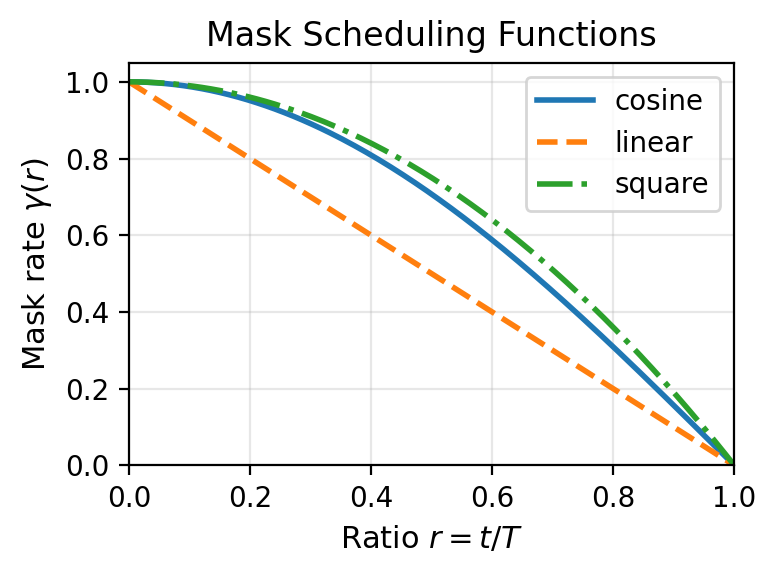
\includegraphics[width=0.85\linewidth]{assets/gamma_curves.png}
	\caption{Mask scheduling functions $\gamma(r)$: fraction of tokens remaining masked as a function of the normalized iteration ratio $r = t/T$.}
	\label{fig:gamma_curves}
\end{figure}

\subsubsection{Mask Evolution in Latent Domain}

\Cref{fig:mask_compare} compares the mask evolution in the $16\times16$ latent space across the three scheduling functions. White pixels indicate masked (unknown) tokens; black pixels indicate predicted (unmasked) tokens.

\begin{figure}[h]
	\centering
	\begin{subfigure}{\linewidth}
		\centering
		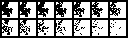
\includegraphics[width=\linewidth]{assets/cosine/mask_0.png}
		\caption{Cosine schedule}
	\end{subfigure}
	\vspace{0.2cm}
	\begin{subfigure}{\linewidth}
		\centering
		\includegraphics[width=\linewidth]{assets/linear/mask_0.png}
		\caption{Linear schedule}
	\end{subfigure}
	\vspace{0.2cm}
	\begin{subfigure}{\linewidth}
		\centering
		\includegraphics[width=\linewidth]{assets/square/mask_0.png}
		\caption{Square schedule}
	\end{subfigure}
	\caption{Mask evolution in the $16\times16$ latent domain over 14 iterations ($t=1$ to $t=14$, left to right). The cosine and square schedules unmask more aggressively in early iterations, while linear progresses at a constant rate.}
	\label{fig:mask_compare}
\end{figure}

\subsubsection{Predicted Image Evolution}

\Cref{fig:imga_compare} shows the corresponding decoded images at each iteration. The first frame is the masked input; subsequent frames show progressive refinement as more tokens are predicted and decoded through the VQGAN decoder.

\begin{figure}[h]
	\centering
	\begin{subfigure}{\linewidth}
		\centering
		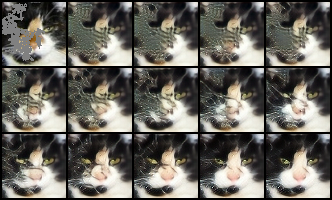
\includegraphics[width=\linewidth]{assets/cosine/imga_0.png}
		\caption{Cosine schedule}
	\end{subfigure}
	\vspace{0.2cm}
	\begin{subfigure}{\linewidth}
		\centering
		\includegraphics[width=\linewidth]{assets/linear/imga_0.png}
		\caption{Linear schedule}
	\end{subfigure}
	\vspace{0.2cm}
	\begin{subfigure}{\linewidth}
		\centering
		\includegraphics[width=\linewidth]{assets/square/imga_0.png}
		\caption{Square schedule}
	\end{subfigure}
	\caption{Predicted images over 15 frames (masked input $\to$ iterations $1$--$14$, left to right, top to bottom). All three schedules converge to similar final quality, but the cosine schedule produces recognizable structure earlier.}
	\label{fig:imga_compare}
\end{figure}

\subsection{Part 2: Best FID Score}

\subsubsection{FID Score Screenshot}
Our best FID score of \textbf{29.11} was achieved with the following settings:
\begin{itemize}
	\item \textbf{Checkpoint}: OneCycleLR best checkpoint (150 epochs, batch size 64)
	\item \textbf{Mask function}: cosine
	\item \textbf{Total iterations}: $T = 10$
	\item \textbf{Sweet spot}: $t^* = 9$
\end{itemize}

\begin{figure}[h]
	\centering
	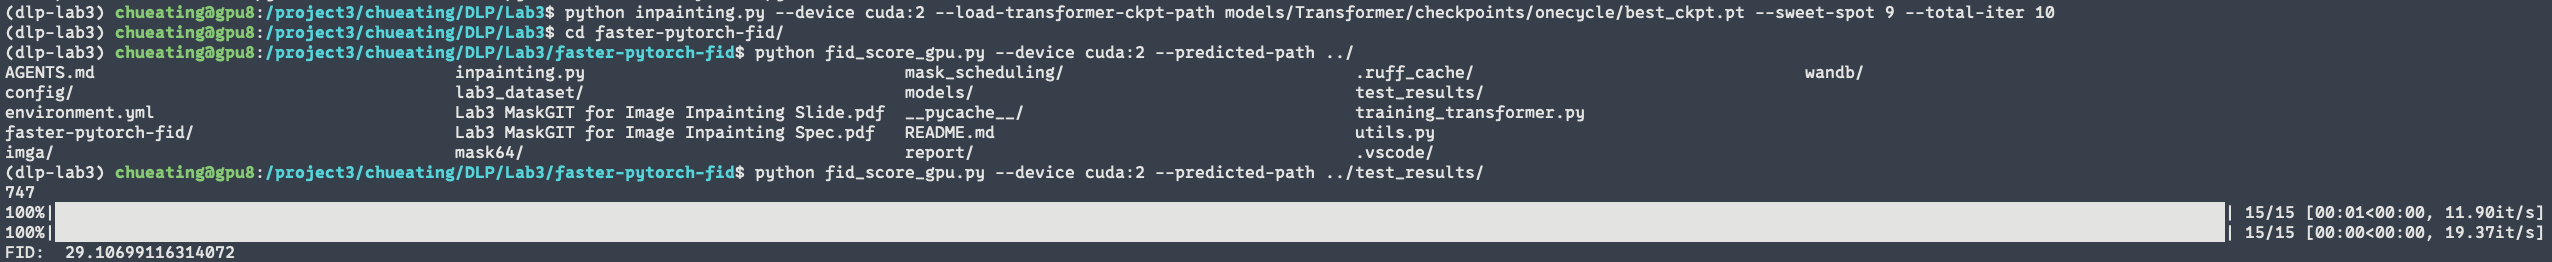
\includegraphics[width=\linewidth]{assets/screenshot.png}
	\caption{FID score screenshot: \textbf{29.11} on 747 test images.}
	\label{fig:fid_screenshot}
\end{figure}

\subsubsection{FID Comparison Across Scheduling Functions}

\begin{table}[h]
	\centering
	\small
	\begin{tabular}{lccc}
		\toprule
		\textbf{Mask Function} & \textbf{$T$} & \textbf{$t^*$} & \textbf{FID $\downarrow$} \\ \midrule
		cosine                 & 10           & 9              & \textbf{29.11}            \\
		linear                 & 10           & 9              & 30.25                     \\
		square                 & 10           & 9              & 29.73                     \\
		\bottomrule
	\end{tabular}
	\caption{FID scores for different mask scheduling functions. All use OneCycleLR checkpoint with $T=10$, $t^*=9$.}
	\label{tab:fid_comparison}
\end{table}

\subsubsection{Masked Images vs.\ Inpainting Results}

\begin{figure}[h]
	\centering
	\begin{subfigure}{0.22\linewidth}
		\centering
		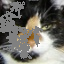
\includegraphics[width=\linewidth]{assets/masked_000.png}
	\end{subfigure}
	\hfill
	\begin{subfigure}{0.22\linewidth}
		\centering
		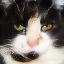
\includegraphics[width=\linewidth]{assets/inpainted_000.png}
	\end{subfigure}
	\hfill
	\begin{subfigure}{0.22\linewidth}
		\centering
		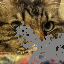
\includegraphics[width=\linewidth]{assets/masked_001.png}
	\end{subfigure}
	\hfill
	\begin{subfigure}{0.22\linewidth}
		\centering
		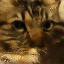
\includegraphics[width=\linewidth]{assets/inpainted_001.png}
	\end{subfigure}

	\vspace{0.2cm}

	\begin{subfigure}{0.22\linewidth}
		\centering
		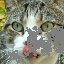
\includegraphics[width=\linewidth]{assets/masked_002.png}
	\end{subfigure}
	\hfill
	\begin{subfigure}{0.22\linewidth}
		\centering
		
\includegraphics[width=\linewidth]{assets/inpainted_002.png}
	\end{subfigure}
	\hfill
	\begin{subfigure}{0.22\linewidth}
		\centering
		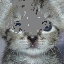
\includegraphics[width=\linewidth]{assets/masked_003.png}
	\end{subfigure}
	\hfill
	\begin{subfigure}{0.22\linewidth}
		\centering
		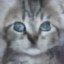
\includegraphics[width=\linewidth]{assets/inpainted_003.png}
	\end{subfigure}

	\caption{Masked input images (left of each pair) and MaskGIT inpainting results (right). The model successfully fills in the gray masked regions with plausible cat face textures.}
	\label{fig:masked_vs_inpainted}
\end{figure}

%------------------------------------------------------------------------

\section{Discussion} \label{sec:discuss}

\subsection{Training Strategy Comparison}

We compared three learning rate schedulers under identical conditions (AdamW, lr${}=10^{-4}$, 150 epochs, batch size 64, gradient accumulation 2).

\begin{figure}[h]
	\centering
	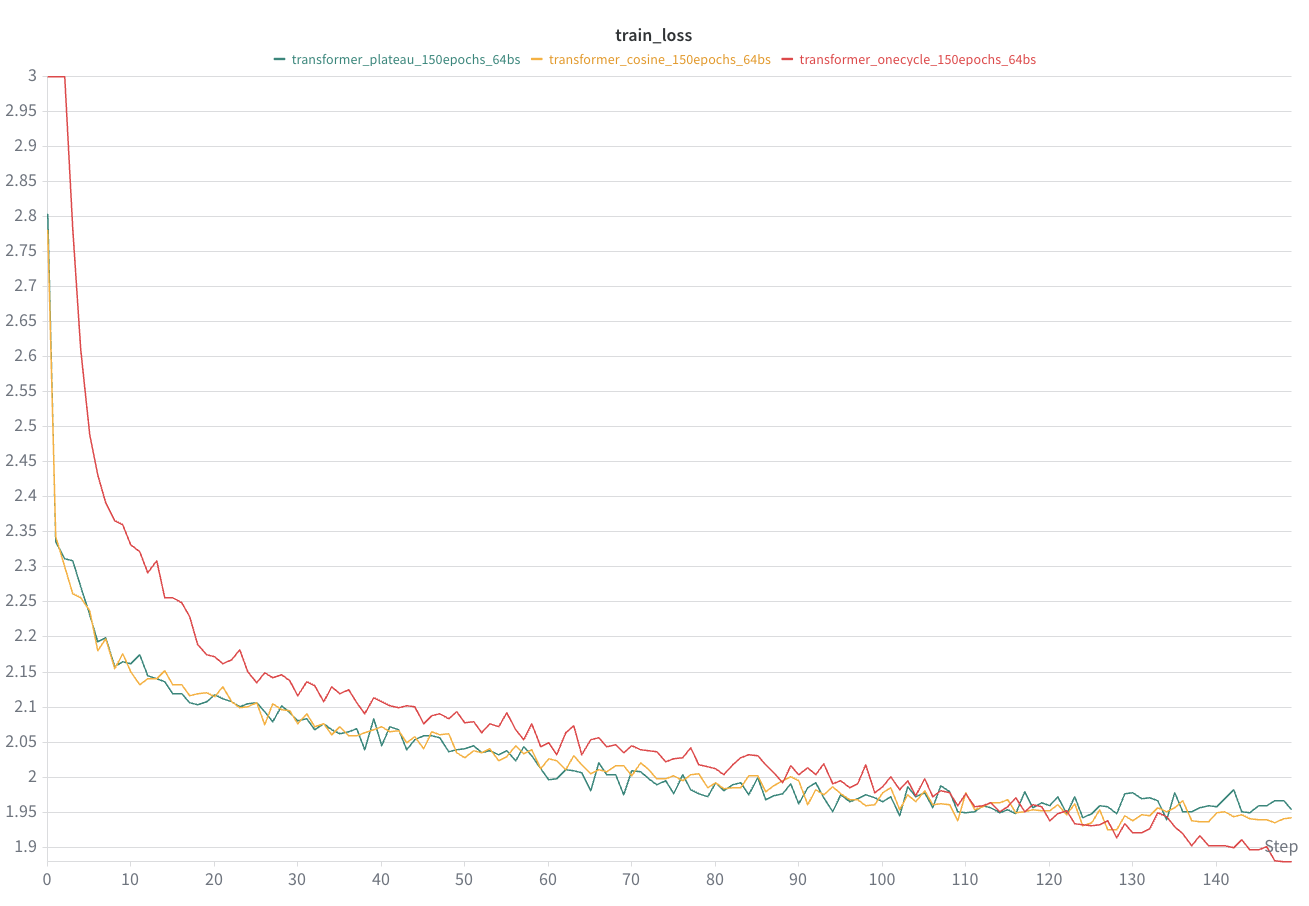
\includegraphics[width=\linewidth]{assets/train_loss.png}
	\caption{Training loss curves for three LR schedulers.}
	\label{fig:train_loss}
\end{figure}

\begin{figure}[h]
	\centering
	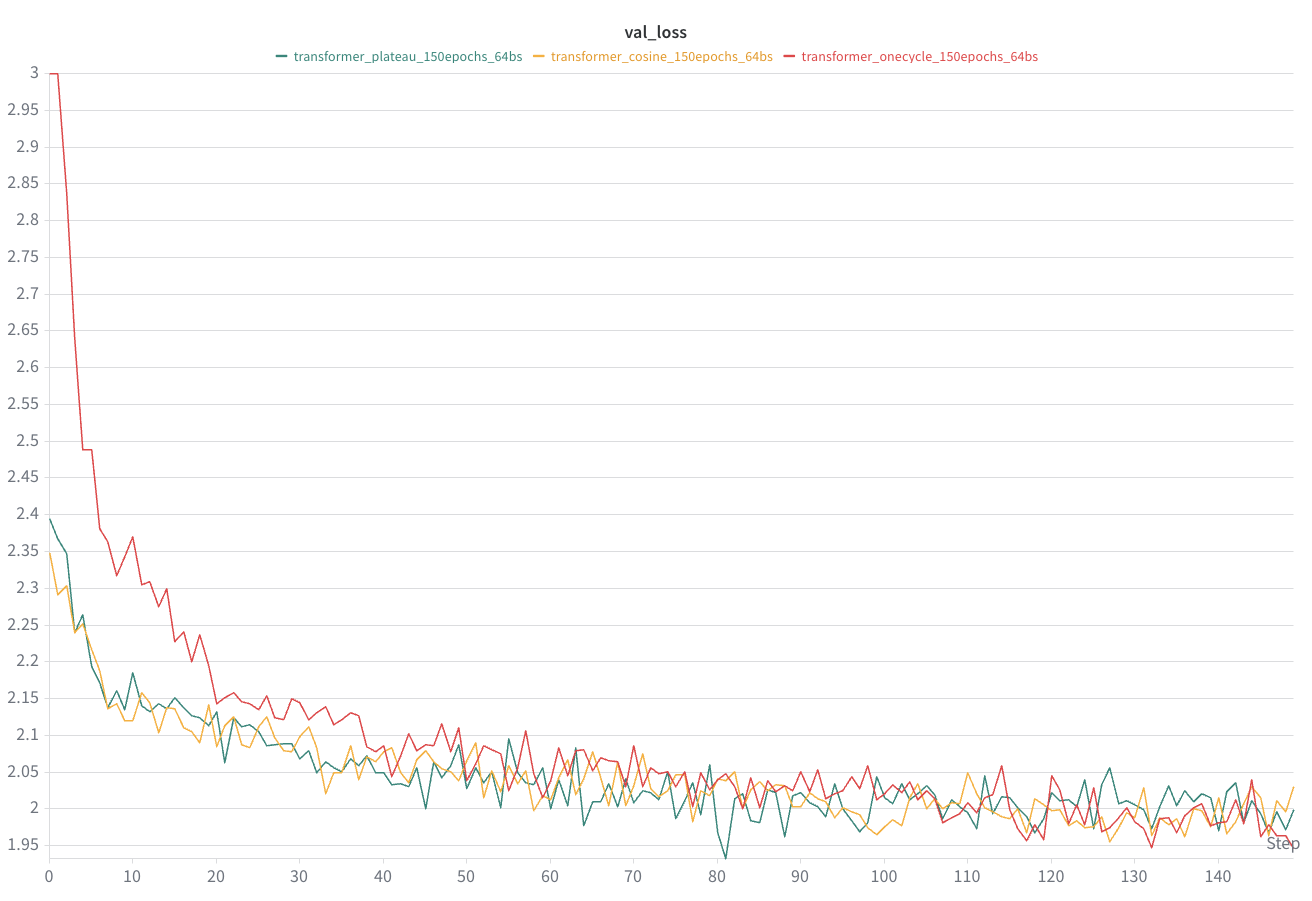
\includegraphics[width=\linewidth]{assets/val_loss.png}
	\caption{Validation loss curves for three LR schedulers.}
	\label{fig:val_loss}
\end{figure}

\begin{figure}[h]
	\centering
	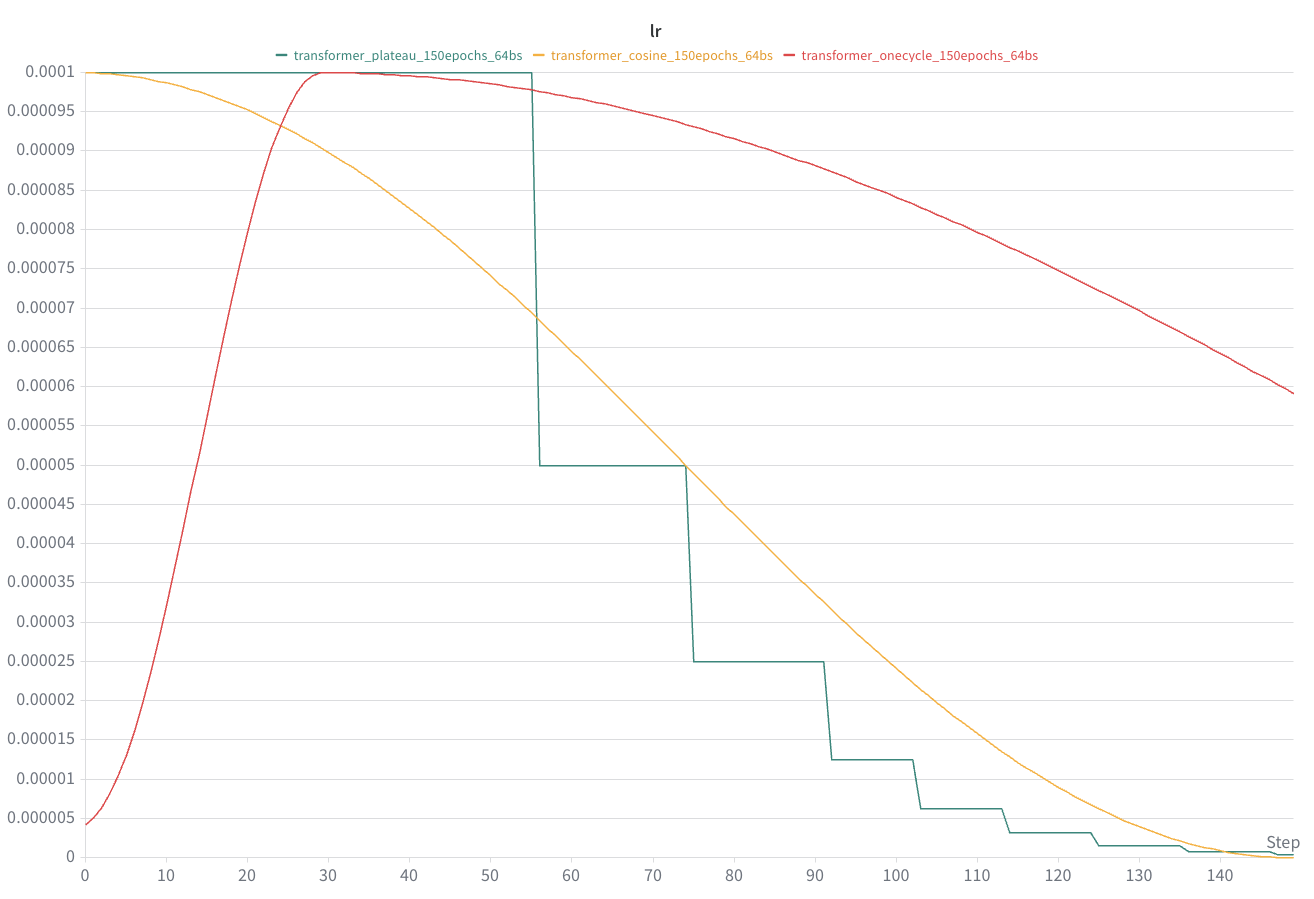
\includegraphics[width=\linewidth]{assets/lr.png}
	\caption{Learning rate schedules over training.}
	\label{fig:lr_schedule}
\end{figure}

\begin{itemize}
	\item \textbf{OneCycleLR} achieved the best validation loss and FID score. The warm-up phase helps the model explore the loss landscape before settling, and the per-batch LR updates provide smoother optimization than per-epoch schedulers.
	\item \textbf{CosineAnnealingLR} performed reasonably but decayed LR to zero by the end, potentially cutting off useful learning in later epochs.
	\item \textbf{ReduceLROnPlateau} reduced LR too aggressively (factor=0.5, patience=10), causing the effective learning rate to drop to near-zero prematurely, resulting in stalled training.
\end{itemize}

\subsection{Sweet Spot and Total Iterations}

We swept $t^*$ (sweet spot) and $T$ (total iterations) to find the optimal decoding configuration. Table~\ref{tab:sweep} summarizes the results.

\begin{table}[h]
	\centering
	\small
	\begin{tabular}{ccc}
		\toprule
		\textbf{$T$} & \textbf{$t^*$} & \textbf{FID $\downarrow$} \\ \midrule
		10           & 5              & 76.98                     \\
		10           & 6              & 55.60                     \\
		10           & 7              & 40.86                     \\
		10           & 8              & 33.03                     \\
		10           & 9              & \textbf{28.94}            \\ \midrule
		15           & 10             & 44.99                     \\
		15           & 11             & 38.30                     \\
		15           & 12             & 32.83                     \\
		15           & 13             & 31.58                     \\
		15           & 14             & 29.02                     \\ \midrule
		20           & 14             & 40.70                     \\
		20           & 16             & 33.28                     \\
		20           & 18             & 31.18                     \\
		20           & 19             & 30.60                     \\
		\bottomrule
	\end{tabular}
	\caption{Sweep of total iterations $T$ and sweet spot $t^*$. Using nearly all iterations ($t^* = T-1$) yields the best FID.}
	\label{tab:sweep}
\end{table}

The clear trend is that using nearly all iterations ($t^* = T - 1$) gives the best FID. Across all three settings, $T=10$ with $t^*=9$ achieves the lowest FID of 28.94. With larger $T$, the cosine schedule spreads unmasking more thinly across more iterations—each step unmasks fewer tokens, giving the model less context per prediction. This increases re-masking noise and error accumulation, resulting in higher FID despite more refinement steps. The $T=15$ results ($t^*=14 \rightarrow$ FID 29.02) are competitive but do not surpass $T=10$.

\subsection{Per-Sample Masking Diversity}

An important implementation detail is sampling the mask ratio $r$ \emph{independently} for each sample in the batch, rather than sharing a single $r$ across the entire batch. This provides the transformer with a more diverse distribution of masking conditions during training, which improves generalization and led to lower validation loss in our experiments.

As shown in \cref{fig:val_loss_r}, the run without per-sample $r$ (green, shared $r$ across the batch) exhibits highly volatile validation loss with large spikes throughout training, whereas per-sample $r$ (orange) converges smoothly and achieves a consistently lower validation loss. The shared-$r$ approach causes entire batches to have the same masking difficulty, leading to high-variance gradients and unstable optimization.

\begin{figure}[h]
	\centering
	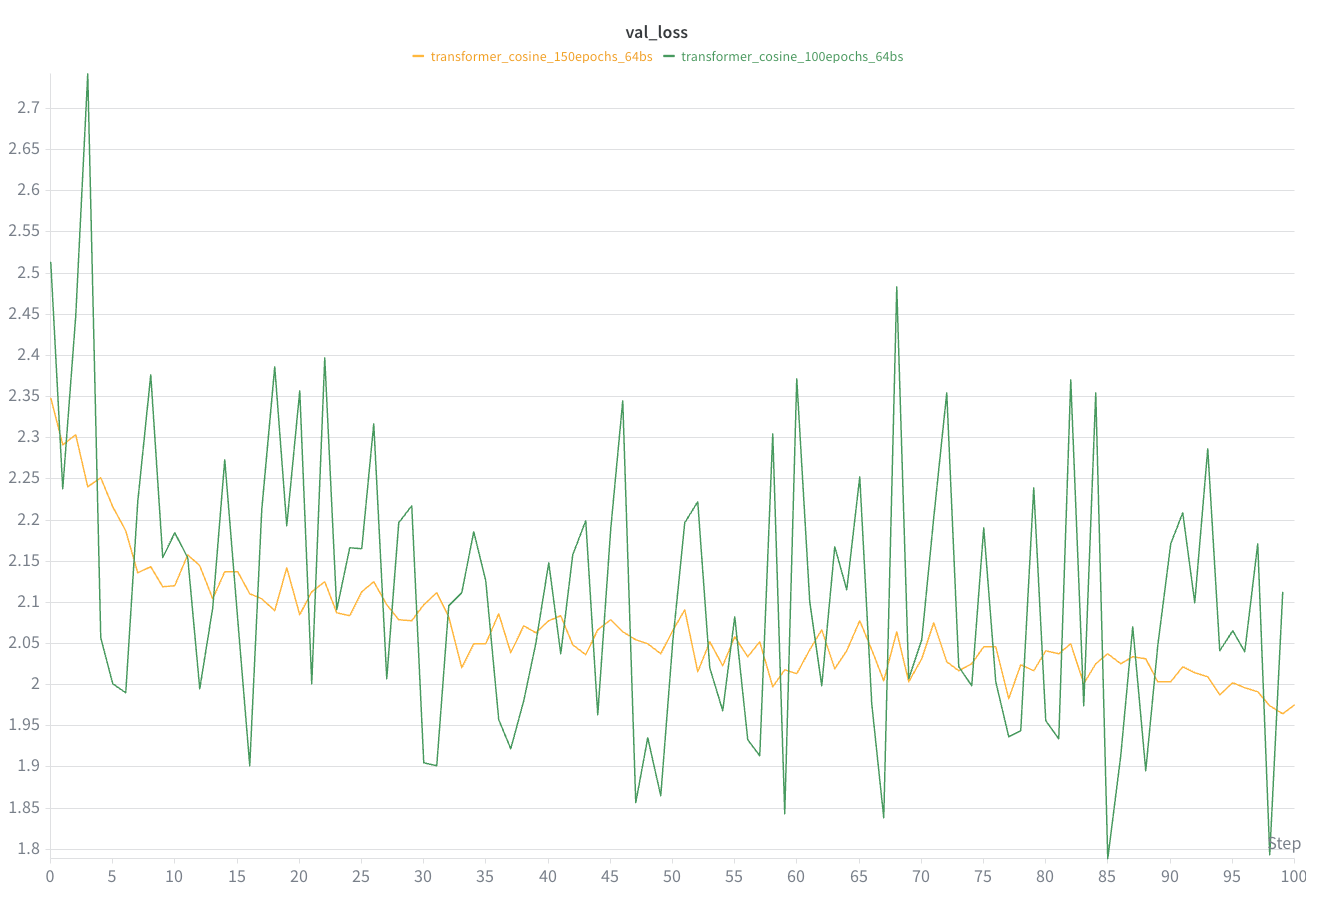
\includegraphics[width=\linewidth]{assets/val_loss_r.png}
	\caption{Validation loss with per-sample $r$ (orange, smooth) vs.\ shared batch-level $r$ (green, noisy). Per-sample masking diversity stabilizes training and yields lower final loss.}
	\label{fig:val_loss_r}
\end{figure}

%%%%%%%%% REFERENCES
{\small
    \bibliographystyle{ieee_fullname}
    \bibliography{egbib}
}

\end{document}
